\chapter{Orbital Molekul Molekul Diatomik}\label{ch:b2:diatomic-mos}

Tuangkan oksigen cair di antara kutub-kutub magnet yang kuat, dan oksigen
itu tertarik ke samping; nitrogen cair jatuh lurus melewatinya. Molekul
oksigen membawa elektron-elektron yang tidak berpasangan, yang ditarik oleh
medan magnet. Struktur Lewisnya, \ce{O=O} dengan setiap elektron
berpasangan, tidak dapat menyatakan hal itu. \omterm{def:b2:diatomic-mos:lcao}{Orbital molekul}, yang dibangun
dari orbital atom pada bab sebelumnya, menempatkan setiap elektron sebuah
molekul pada tingkat energinya sendiri: \omterm{def:b2:diatomic-mos:lcao}{orbital molekul} menjelaskan
kemagnetan oksigen, kekuatan dan panjang ikatan, serta energi yang
diperlukan untuk mengionisasi molekul --- dan meletakkan dasar bagi
kereaktifan dalam bab-bab berikutnya.

\begin{recall}
\Cref{ch:b2:atomic-orbitals}: orbital atom, bentuk, tanda, dan energinya.
Jilid Tahun 1: struktur Lewis, ikatan $\sigma$ dan $\pi$ sebagai pengertian
deskriptif, hibridisasi dan batas-batasnya, elektron tak berpasangan dan
radikal.
\end{recall}

\begin{omfigure}
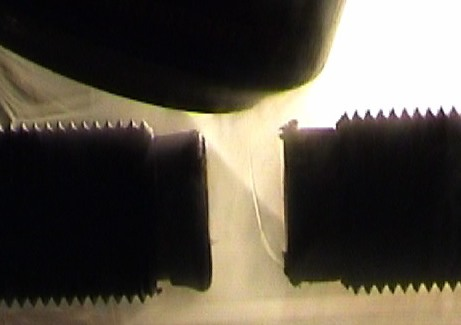
\includegraphics[width=0.42\linewidth]{images/book3/liquid-oxygen.jpg}

{\small Aliran tipis oksigen cair, yang jatuh di antara kutub-kutub magnet
yang kuat, tertarik ke arah kutub-kutub itu dan menggantung seperti
jembatan: molekulnya \omterm{def:b2:diatomic-mos:magnetism}{paramagnetik}. (Foto: Pieter Kuiper, domain publik,
Wikimedia Commons.)}
\end{omfigure}

\section{Metode LCAO}

\begin{definition}[Orbital molekul]\label{def:b2:diatomic-mos:lcao}
Yang disebut \emph{orbital molekul}\index{orbital molekul} adalah \omterm{def:b2:atomic-orbitals:wavefunction}{fungsi
gelombang} satu elektron dalam sebuah molekul, yang tersebar di atas semua
intinya. Dalam metode \emph{LCAO}\index{LCAO} (kombinasi linear orbital
atom), orbital itu dituliskan sebagai jumlah orbital-orbital atom dari
atom-atomnya, $\psi = \sum_i c_i\varphi_i$, dengan koefisien yang dipilih
agar energinya paling rendah.
\end{definition}

Untuk dua atom A dan B, yang masing-masing membawa satu orbital,
$\psi = c_A\varphi_A + c_B\varphi_B$. Energi elektron dalam $\psi$, yang
diminimumkan terhadap koefisien-koefisiennya, melibatkan tiga bilangan.

\begin{definition}[Integral-integral metode LCAO]\label{def:b2:diatomic-mos:integrals}
Untuk dua orbital atom real $\varphi_A$, $\varphi_B$ dan operator energi $\hat H$
elektron dalam molekul:
\begin{itemize}
  \item \emph{integral tumpang-tindih}\index{integral tumpang-tindih}
        $S = \int\varphi_A\varphi_B\,dV$ mengukur seberapa banyak kedua
        orbital menempati daerah yang sama ($S = 1$ untuk orbital-orbital
        identik yang saling menutupi);
  \item \emph{integral Coulomb}\index{integral Coulomb} $\alpha_A = \int\varphi_A\hat
        H\varphi_A\,dV$ adalah energi elektron dalam $\varphi_A$ di dalam
        molekul, yang mendekati \omterm{def:b2:atomic-orbitals:orbital-energy}{energi orbital} atom itu;
  \item \emph{integral resonansi}\index{integral resonansi} $\beta = \int\varphi_A\hat
        H\varphi_B\,dV$, yang negatif, mengukur kopling kedua orbital.
\end{itemize}
Energi-energi $E$ \omterm{def:b2:diatomic-mos:lcao}{orbital molekul} adalah akar-akar \emph{determinan
sekular}\index{determinan sekular}
\[
  \begin{vmatrix} \alpha_A - E & \beta - ES \\ \beta - ES & \alpha_B - E \end{vmatrix} = 0 .
\]
\end{definition}

Determinan itu berasal dari peminimuman
$E = \int\psi\hat H\psi\,dV/\int\psi^2\,dV$ terhadap $c_A$ dan $c_B$: kedua
syarat $\partial E/\partial c_A =
\partial E/\partial c_B = 0$ membentuk
sistem linear homogen, yang hanya mempunyai penyelesaian tak nol jika
determinannya nol. Langkah variasional itu di sini diterima tanpa bukti.

\begin{theorem}[Dua orbital identik]\label{thm:b2:diatomic-mos:homonuclear}
Untuk $\alpha_A = \alpha_B = \alpha$, kedua \omterm{def:b2:diatomic-mos:lcao}{orbital molekulnya} adalah
\[
  E_+ = \frac{\alpha + \beta}{1 + S}, \quad \psi_+ = \frac{\varphi_A + \varphi_B}{\sqrt{2(1 + S)}} ;
  \qquad
  E_- = \frac{\alpha - \beta}{1 - S}, \quad \psi_- = \frac{\varphi_A - \varphi_B}{\sqrt{2(1 - S)}} .
\]
\end{theorem}

\begin{proof}
Determinan itu memberikan $(\alpha - E)^2 = (\beta - ES)^2$, sehingga
$\alpha - E = \pm(\beta - ES)$. Dengan tanda plus, $E(1 + S) = \alpha + \beta$;
dengan tanda minus, $E(1 - S) = \alpha
- \beta$. Kembali ke sistem linear,
$(\alpha - E)c_A + (\beta - ES)c_B = 0$ memberikan $c_B
= c_A$ untuk $E_+$
dan $c_B = -c_A$ untuk $E_-$. Normalisasi: $\int(\varphi_A \pm
\varphi_B)^2\,dV = 2 \pm 2S$.
\end{proof}

\begin{definition}[Orbital ikatan dan orbital antiikatan]\label{def:b2:diatomic-mos:bonding}
Yang disebut \emph{orbital ikatan}\index{orbital ikatan} adalah orbital yang
terletak di bawah orbital-orbital atom pembentuknya: kerapatan elektronnya
menumpuk di antara inti-inti. Yang disebut \emph{orbital
antiikatan}\index{orbital antiikatan} terletak di atasnya dan mempunyai
bidang simpul di antara inti-inti. Yang disebut \emph{orbital
nonikatan}\index{orbital nonikatan} mempertahankan \omterm{def:b2:atomic-orbitals:orbital-energy}{energi orbital} atom,
yang tidak menemukan pasangan untuk bergabung.
\end{definition}

\begin{proposition}[Orbital antiikatan naik lebih jauh]\label{prop:b2:diatomic-mos:asymmetry}
Untuk $S > 0$, tingkat antiikatan terangkat di atas $\alpha$ lebih jauh
daripada tingkat ikatan turun di bawahnya.
\end{proposition}

\begin{proof}
$E_+ - \alpha = (\beta - \alpha S)/(1 + S)$ dan
$E_- - \alpha = -(\beta - \alpha S)/(1 - S)$. Pembilang $\beta - \alpha S$
negatif (koplingnya dominan), dan $1 - S < 1
+ S$: pergeseran kedua lebih
besar nilainya.
\end{proof}

Dengan dua elektron, seperti pada \ce{H2}, keduanya masuk ke $\psi_+$ dan
molekul itu lebih stabil daripada atom-atom yang terpisah. Dengan empat,
seperti pada \ce{He2}, dua elektron harus masuk ke $\psi_-$, yang
menuntut lebih banyak daripada yang diperoleh $\psi_+$: \ce{He2} tidak
terikat.

\begin{omfigure}
\begin{MOdiagram}[names, labels]
  \atom[H]{left}{ 1s = {0;up} }
  \atom[H]{right}{ 1s = {0;up} }
  \molecule[\ce{H2}]{ 1sMO = {.75;pair} }
\end{MOdiagram}
\hspace{1.5cm}
\begin{MOdiagram}[names, labels]
  \atom[He]{left}{ 1s = {0;pair} }
  \atom[He]{right}{ 1s = {0;pair} }
  \molecule[\ce{He2}]{ 1sMO = {.75;pair,pair} }
\end{MOdiagram}

{\small Diagram \omterm{def:b2:diatomic-mos:lcao}{orbital molekul} \ce{H2} (\omterm{def:b2:diatomic-mos:bond-order}{orde ikatan} 1) dan \ce{He2} (\omterm{def:b2:diatomic-mos:bond-order}{orde
ikatan} 0, tidak terikat). Setiap kotak adalah sebuah tingkat yang memuat
paling banyak dua elektron dengan spin berlawanan; garis putus-putus
menghubungkan setiap \omterm{def:b2:diatomic-mos:lcao}{orbital molekul} dengan orbital-orbital atom
pembentuknya.}
\end{omfigure}

\section{Tumpang-tindih dan simetri}

\begin{definition}[Orbital $\sigma$ dan $\pi$]\label{def:b2:diatomic-mos:sigma-pi}
Sebuah \emph{orbital $\sigma$}\index{orbital sigma@orbital $\sigma$} molekul
linear tidak berubah oleh rotasi apa pun di sekitar sumbu molekul: orbital
itu tidak mempunyai bidang simpul yang memuat sumbu. Sebuah
\emph{orbital $\pi$}\index{orbital pi@orbital $\pi$} berganti tanda pada
rotasi $180^\circ$ di sekitar sumbu: orbital itu mempunyai satu bidang simpul
yang memuat sumbu. Tanda bintang menandai orbital-orbital antiikatan
($\sigma^*$, $\pi^*$).
\end{definition}

\begin{proposition}[Tumpang-tindih nol karena simetri]\label{prop:b2:diatomic-mos:symmetry}
Dua orbital yang satu simetris dan yang lain antisimetris terhadap sebuah
bidang yang memuat sumbu molekul mempunyai tumpang-tindih nol dan \omterm{def:b2:diatomic-mos:integrals}{integral
resonansi} nol: keduanya tidak bergabung.
\end{proposition}

\begin{proof}
Pencerminan terhadap bidang itu tidak mengubah ruang tetapi mengubah hasil
kali $\varphi_A\varphi_B$ menjadi lawannya di titik bayangan: sumbangan kedua
belahan ruang pada $\int\varphi_A\varphi_B\,dV$ saling meniadakan. Hal yang sama
berlaku untuk $\int\varphi_A\hat H\varphi_B\,dV$, karena $\hat H$ mempunyai
simetri molekul.
\end{proof}

Dua orbital berinteraksi kuat jika keduanya mempunyai simetri yang sama
(tumpang-tindih tak nol), bertumpang-tindih dengan baik, dan terletak pada
energi yang berdekatan. Orbital 1s satu atom dan orbital $2\mathrm p_x$ atom
lainnya ($x$ tegak lurus sumbu) tidak pernah bergabung; orbital-orbital
$2\mathrm p_z$ (sepanjang sumbu) menghasilkan orbital $\sigma$; $2\mathrm p_x$
dan $2\mathrm p_y$ menghasilkan dua pasang orbital $\pi$ yang energinya sama.

\begin{omfigure}
\begin{tikzpicture}[font=\small]
  % sigma 1s
  \pic at (0,0) {oms={0.85}}; \pic at (0.7,0) {oms={0.85}};
  \node at (0.35,-0.75) {$\sigma_{1s}$};
  \pic at (2.2,0) {oms={0.85}}; \pic at (2.9,0) {oms={-0.85}};
  \node at (2.55,-0.75) {$\sigma^*_{1s}$};
  % sigma 2p
  \pic at (4.6,0) {omp={-1}{0}}; \pic at (5.6,0) {omp={1}{0}};
  \node at (5.1,-0.75) {$\sigma_{2p}$};
  \pic at (7.4,0) {omp={-1}{0}}; \pic at (8.6,0) {omp={-1}{0}};
  \node at (8.0,-0.75) {$\sigma^*_{2p}$};
  % pi 2p
  \pic at (10.2,0) {omp={1}{90}}; \pic at (10.9,0) {omp={1}{90}};
  \node at (10.55,-0.95) {$\pi_{2p}$};
  \pic at (12.2,0) {omp={1}{90}}; \pic at (12.9,0) {omp={-1}{90}};
  \node at (12.55,-0.95) {$\pi^*_{2p}$};
  \draw[black!40, dashed] (-0.6,0) -- (13.4,0);
\end{tikzpicture}

{\small Orbital-orbital molekul diatomik homonuklir, skematis (sumbu molekul
mendatar dan putus-putus). Kombinasi sefase (ikatan) mengumpulkan warna
yang sama di antara inti-inti; kombinasi berlawanan fase (antiikatan)
menempatkan bidang simpul di antara keduanya. Orbital $\sigma$ simetris
terhadap sumbu; setiap orbital $\pi$ mempunyai sumbu itu pada bidang
simpulnya.}
\end{omfigure}

\section{Molekul diatomik homonuklir periode 2}

Dengan orbital 2s dan 2p dua atom periode 2, terbentuk delapan \omterm{def:b2:diatomic-mos:lcao}{orbital
molekul}: $\sigma_{2s}$, $\sigma^*_{2s}$, $\sigma_{2p}$, dua $\pi_{2p}$, dua
$\pi^*_{2p}$, $\sigma^*_{2p}$.

\begin{proposition}[Pencampuran s--p]\label{prop:b2:diatomic-mos:sp-mixing}
Untuk \ce{O2} dan \ce{F2}, urutannya adalah $\sigma_{2s} < \sigma^*_{2s} < \sigma_{2p} < \pi_{2p} <
\pi^*_{2p} < \sigma^*_{2p}$. Untuk \ce{Li2} sampai \ce{N2}, yang tingkat 2s
dan 2p-nya berdekatan, orbital-orbital $\sigma$ yang dibuat dari 2s dan
$2\mathrm p_z$ bercampur: $\sigma_{2p}$ terdorong ke atas $\pi_{2p}$.
\end{proposition}

\begin{proof}[Argumen]
Orbital $\sigma_{2s}$ dan $\sigma_{2p}$ mempunyai simetri yang sama dan dapat
bergabung satu sama lain. Dua tingkat dengan simetri yang sama saling
menolak (\cref{thm:b2:diatomic-mos:heteronuclear} di bawah): $\sigma_{2s}$
turun, $\sigma_{2p}$ naik, makin kuat makin dekat keduanya. Selisih 2s--2p
bertambah sepanjang periode, sehingga pengaruhnya besar di kiri dan kecil
untuk oksigen dan fluor. Persilangan antara nitrogen dan oksigen diterima
dari spektrum fotoelektron yang terukur.
\end{proof}

\begin{definition}[Orde ikatan]\label{def:b2:diatomic-mos:bond-order}
Yang disebut \emph{orde ikatan}\index{orde ikatan} molekul diatomik adalah
$b = (n_b -
n_a)/2$, dengan $n_b$ dan $n_a$ jumlah elektron dalam \omterm{def:b2:diatomic-mos:bonding}{orbital
ikatan} dan \omterm{def:b2:diatomic-mos:bonding}{orbital antiikatan}.
\end{definition}

\begin{proposition}[Orde ikatan dan ikatan]\label{prop:b2:diatomic-mos:bond-order}
Di antara atom-atom dari pasangan unsur yang sama, \omterm{def:b2:diatomic-mos:bond-order}{orde ikatan} yang lebih
tinggi disertai ikatan yang lebih pendek dan lebih kuat; \omterm{def:b2:diatomic-mos:bond-order}{orde ikatan} nol
berarti tidak ada ikatan.
\end{proposition}

\begin{proof}[Argumen]
Setiap elektron ikatan menambah kerapatan di antara inti-inti dan
menurunkan energi; setiap elektron antiikatan mengurangi kerapatan itu dan
menaikkan energi paling sedikit sebesar itu pula
(\cref{prop:b2:diatomic-mos:asymmetry}). Jumlah bersih pasangan ikatan
mengukur pengikatannya. Perbandingan ini hanya bermakna untuk atom-atom
yang serupa: \ce{Li2} mempunyai \omterm{def:b2:diatomic-mos:bond-order}{orde ikatan} 1 seperti \ce{F2}, tetapi
orbital-orbital 2s-nya jauh lebih besar.
\end{proof}

\begin{definition}[Paramagnetik dan diamagnetik]\label{def:b2:diatomic-mos:magnetism}
Sebuah zat disebut \emph{paramagnetik}\index{paramagnetik} jika molekulnya
mempunyai elektron tak berpasangan: zat itu tertarik ke dalam medan
magnet. Zat itu disebut \emph{diamagnetik}\index{diamagnetik} jika semua
elektronnya berpasangan: zat itu sedikit terdorong keluar dari medan.
\end{definition}

\begin{omfigure}
\begin{MOdiagram}[names, labels, style=square, distance=4.2cm, labels-fs=\scriptsize]
  \atom[N]{left}{ 2s = {0;pair}, 2p = {3.5;up,up,up} }
  \atom[N]{right}{ 2s = {0;pair}, 2p = {3.5;up,up,up} }
  \molecule[\ce{N2}]{ 2sMO = {.7;pair,pair}, 2pMO = {0.4/2.5,1.4;pair,pair,pair} }
\end{MOdiagram}
\hfill
\begin{MOdiagram}[names, labels, style=square, distance=4.2cm, labels-fs=\scriptsize]
  \atom[O]{left}{ 2s = {0;pair}, 2p = {3.5;pair,up,up} }
  \atom[O]{right}{ 2s = {0;pair}, 2p = {3.5;pair,up,up} }
  \molecule[\ce{O2}]{ 2sMO = {.7;pair,pair}, 2pMO = {1.8,.8;pair,pair,pair,up,up} }
\end{MOdiagram}

{\small Diagram \omterm{def:b2:diatomic-mos:lcao}{orbital molekul} valensi \ce{N2} (kiri, dengan pencampuran
s--p: $\sigma_{2p}$ di atas $\pi_{2p}$) dan \ce{O2} (kanan). Nitrogen: \omterm{def:b2:diatomic-mos:bond-order}{orde
ikatan} $(8 - 2)/2 = 3$, semua elektron berpasangan. Oksigen: \omterm{def:b2:diatomic-mos:bond-order}{orde ikatan}
$(8 - 4)/2 = 2$, dengan dua elektron tak berpasangan dalam kedua orbital
$\pi^*$ (aturan Hund): \ce{O2} \omterm{def:b2:diatomic-mos:magnetism}{paramagnetik}. Diagram-diagram ini mengambil
$x$ sebagai sumbu molekul, sehingga labelnya $2\sigma_x$, $2\pi_y$,
$2\pi_z$.}
\end{omfigure}

\begin{method}[Membangun dan mengisi diagram OM]\label{met:b2:diatomic-mos:build-diagram}
\begin{enumerate}
  \item Letakkan orbital-orbital atom valensi setiap atom pada energinya,
        dengan atom yang lebih elektronegatif di bawah.
  \item Gabungkan orbital-orbital yang simetrinya sama: setiap pasangan
        menghasilkan satu \omterm{def:b2:diatomic-mos:bonding}{orbital ikatan} di bawah dan satu \omterm{def:b2:diatomic-mos:bonding}{orbital
        antiikatan} di atas; orbital tanpa pasangan tetap nonikatan.
  \item Untuk molekul homonuklir periode 2, pakailah urutan dengan
        $\sigma_{2p}$ di atas $\pi_{2p}$ sampai nitrogen, dan di bawahnya
        mulai dari oksigen.
\end{enumerate}
\end{method}

\begin{method}[Membaca diagram yang terisi]\label{met:b2:diatomic-mos:fill}
\begin{enumerate}
  \item Hitunglah elektron valensi (tambahkan satu untuk setiap muatan
        negatif, kurangi satu untuk setiap muatan positif).
  \item Isilah dari bawah, dua per orbital, dengan aturan Hund untuk
        tingkat-tingkat yang terdegenerasi.
  \item \omterm{def:b2:diatomic-mos:bond-order}{Orde ikatan} $(n_b - n_a)/2$; elektron tak berpasangan memberikan
        paramagnetisme.
  \item Tingkat terisi tertinggi adalah yang pertama terionisasi.
\end{enumerate}
\end{method}

\begin{omfigure}
\small
\renewcommand{\arraystretch}{1.15}
\begin{tabular}{lcccccc}
 & \ce{Li2} & \ce{C2} & \ce{N2} & \ce{O2} & \ce{F2} & \ce{NO} \\ \hline
elektron valensi & 2 & 8 & 10 & 12 & 14 & 11 \\
\omterm{def:b2:diatomic-mos:bond-order}{orde ikatan} & 1 & 2 & 3 & 2 & 1 & 2.5 \\
elektron tak berpasangan & 0 & 0 & 0 & 2 & 0 & 1 \\
panjang ikatan $r_e$ (pm) & 267.3 & 124.3 & 109.8 & 120.8 & 141.2 & 115.1 \\
$D_0$ (\unit{eV}) & 1.04 & 6.15 & 9.76 & 5.12 & 1.60 & 6.51 \\
\end{tabular}

\smallskip
{\small Molekul diatomik periode 2: \omterm{def:b2:diatomic-mos:bond-order}{orde ikatan} dari diagram OM; panjang
ikatan dari spektroskopi, energi disosiasi $D_0$ dari entalpi pembentukan
yang ditabelkan pada \qty{0}{K}, $D_0 = \Delta_f H_0(\mathrm A) + \Delta_f H_0(\mathrm B) - \Delta_f
H_0(\mathrm{AB})$.}
% ledger: re:Li2, re:C2, re:N2, re:O2, re:F2, re:NO, janafH0:Li, janafH0:Li2, janafH0:C, janafH0:C2, janafH0:N, janafH0:O, janafH0:F, janafH0:NO
\end{omfigure}

\section{Molekul diatomik heteronuklir}

\begin{theorem}[Dua orbital dengan energi berbeda]\label{thm:b2:diatomic-mos:heteronuclear}
Untuk $\alpha_A > \alpha_B$ (B lebih elektronegatif), dengan $S$ diabaikan,
$\bar\alpha = (\alpha_A
+ \alpha_B)/2$ dan $\Delta = \alpha_A - \alpha_B$:
\[
  E_\mp = \bar\alpha \mp \sqrt{\Delta^2/4 + \beta^2} .
\]
\omterm{def:b2:diatomic-mos:bonding}{Orbital ikatan} (yang lebih rendah) mempunyai koefisien yang lebih besar
pada B, \omterm{def:b2:diatomic-mos:bonding}{orbital antiikatan} pada A; jika $\Delta \gg |\beta|$,
$E_- \approx \alpha_B - \beta^2/\Delta$ dan $E_+
\approx \alpha_A + \beta^2/\Delta$.
\end{theorem}

\begin{proof}
Dengan $S = 0$, energi-energinya adalah nilai-nilai eigen
$\begin{pmatrix}\alpha_A & \beta \\
\beta & \alpha_B\end{pmatrix}$: $(\alpha_A - E)(\alpha_B - E) = \beta^2$,
yang akar-akarnya $\bar\alpha \pm \sqrt{\Delta^2/4 + \beta^2}$. Untuk akar
yang lebih rendah, $(\alpha_B - E_-)c_B = -\beta
c_A$;
$\alpha_B - E_- = \sqrt{\Delta^2/4 + \beta^2} - \Delta/2$ lebih kecil
daripada $|\beta|$, sehingga $|c_A| < |c_B|$. Untuk $\Delta \gg |\beta|$,
$\sqrt{\Delta^2/4 + \beta^2} \approx \Delta/2 +
\beta^2/\Delta$.
\end{proof}

\begin{omfigure}
\begin{tikzpicture}
\begin{axis}[width=0.55\linewidth, height=6cm, xmin=0, xmax=8, ymin=-5, ymax=5,
  axis x line=bottom, axis y line=left, xlabel={$\Delta/|\beta|$}, ylabel={$E/|\beta|$},
  tick label style={font=\small}, label style={font=\small}]
\addplot[omThm, thick] table[x=d, y=Ehigh] {figdata/out/bachelor-2-two-level-a.dat};
\addplot[omDef, thick] table[x=d, y=Elow] {figdata/out/bachelor-2-two-level-a.dat};
\addplot[black!50, densely dotted] table[x=d, y=aA] {figdata/out/bachelor-2-two-level-a.dat};
\addplot[black!50, densely dotted] table[x=d, y=aB] {figdata/out/bachelor-2-two-level-a.dat};
\addplot[omThm, dashed] table[x=d, y=Phigh] {figdata/out/bachelor-2-two-level-a-pert.dat};
\addplot[omDef, dashed] table[x=d, y=Plow] {figdata/out/bachelor-2-two-level-a-pert.dat};
\node[font=\scriptsize, black!60, anchor=north west] at (axis cs:5.5,2.6) {$\alpha_A$};
\node[font=\scriptsize, black!60, anchor=south west] at (axis cs:5.5,-2.6) {$\alpha_B$};
\node[font=\scriptsize, omThm, anchor=south east] at (axis cs:3.2,2.2) {antiikatan};
\node[font=\scriptsize, omDef, anchor=north east] at (axis cs:3.2,-2.2) {ikatan};
\end{axis}
\end{tikzpicture}

{\small Dua tingkat yang berinteraksi. Ketika selisih $\Delta$ antara
orbital-orbital atom bertambah, tingkat-tingkat molekul (garis penuh)
mendekati tingkat-tingkat atom (titik-titik): stabilisasi $\beta^2/\Delta$
pada limit perturbatif (putus-putus) menjadi kecil. Pada $\Delta = 0$,
pemisahannya $2|\beta|$.}
\end{omfigure}

Dalam hidrogen fluorida, orbital 1s hidrogen bertemu dengan orbital-orbital
2p fluor yang jauh lebih rendah. Hanya $2\mathrm p_z$, sepanjang sumbu, yang
mempunyai simetri yang tepat: orbital itu membentuk \omterm{def:b2:diatomic-mos:bonding}{orbital ikatan} $\sigma$
yang berbobot pada fluor, dan orbital $\sigma^*$ yang berbobot pada
hidrogen. Orbital $2\mathrm p_x$ dan $2\mathrm p_y$ fluor tetap nonikatan:
keduanya adalah pasangan elektron bebasnya. Ikatannya terpolarisasi ke
arah fluor.

Karbon monoksida mempunyai sepuluh elektron valensi seperti \ce{N2} dan
diagram yang serupa, tetapi orbital-orbital oksigennya terletak lebih
rendah. Orbital-orbital ikatannya berbobot pada oksigen; orbital terisi
tertingginya, sebuah orbital $\sigma$ yang berbobot pada karbon, adalah
pasangan elektron bebas pada karbon. Karena itu karbon monoksida terikat
pada logam melalui karbon (\cref{ch:b2:coordination-complexes}).

\begin{omfigure}
\begin{tikzpicture}[font=\small]
  % CO schematic: C left (higher), O right (lower)
  \pic (c2s) at (0,0.6) {omlevel={ud}{0.8}}; \node[left] at (-0.5,0.6) {2s};
  \pic (c2p1) at (-0.45,2.6) {omlevel={u}{0.4}}; \pic (c2p2) at (0,2.6) {omlevel={u}{0.4}}; \pic (c2p3) at (0.45,2.6) {omlevel={empty}{0.4}};
  \node[left] at (-0.75,2.6) {2p};
  \node at (0,-0.6) {C};
  \pic (o2s) at (6,-1.2) {omlevel={ud}{0.8}}; \node[right] at (6.5,-1.2) {2s};
  \pic (o2p1) at (5.55,1.4) {omlevel={ud}{0.4}}; \pic (o2p2) at (6,1.4) {omlevel={u}{0.4}}; \pic (o2p3) at (6.45,1.4) {omlevel={u}{0.4}};
  \node[right] at (6.75,1.4) {2p};
  \node at (6,-2.2) {O};
  % MOs
  \pic (m1) at (3,-1.8) {omlevel={ud}{0.8}};
  \pic (m2) at (3,-0.2) {omlevel={ud}{0.8}};
  \pic (m3a) at (2.75,0.9) {omlevel={ud}{0.45}}; \pic (m3b) at (3.25,0.9) {omlevel={ud}{0.45}};
  \pic (m4) at (3,1.9) {omlevel={ud}{0.8}};
  \pic (m5a) at (2.75,3.3) {omlevel={empty}{0.45}}; \pic (m5b) at (3.25,3.3) {omlevel={empty}{0.45}};
  \pic (m6) at (3,4.4) {omlevel={empty}{0.8}};
  \draw[omcorr, densely dashed] (c2s-r) -- (m1-l) (o2s-l) -- (m1-r);
  \draw[omcorr, densely dashed] (c2s-r) -- (m2-l) (o2s-l) -- (m2-r);
  \draw[omcorr, densely dashed] (c2p3-r) -- (m3a-l) (o2p1-l) -- (m3b-r);
  \draw[omcorr, densely dashed] (c2p3-r) -- (m4-l) (o2p1-l) -- (m4-r);
  \draw[omcorr, densely dashed] (c2p3-r) -- (m5a-l) (o2p1-l) -- (m5b-r);
  \draw[omcorr, densely dashed] (c2p3-r) -- (m6-l) (o2p1-l) -- (m6-r);
  \node[omsymlabel, below=0.17cm, inner sep=0.5pt] at (m1-c) {$\sigma$};
  \node[omsymlabel, below=0.17cm, inner sep=0.5pt] at (m2-c) {$\sigma$};
  \node[omsymlabel, below=0.17cm, inner sep=0.5pt] at (3,0.9) {$\pi$};
  \node[omsymlabel, below=0.24cm, inner sep=0.5pt] at (m4-c) {$\sigma$ (PEB C)};
  \node[omsymlabel, below=0.05cm, inner sep=0.5pt] at (3,3.3) {$\pi^*$};
  \node[omsymlabel, below=0.05cm, inner sep=0.5pt] at (m6-c) {$\sigma^*$};
  \node at (3,-2.6) {CO};
\end{tikzpicture}

{\small Orbital-orbital valensi karbon monoksida, skematis: orbital-orbital
oksigen terletak lebih rendah daripada orbital-orbital karbon. \omterm{def:b2:diatomic-mos:bond-order}{Orde ikatan}
3 seperti pada \ce{N2}; orbital terisi tertinggi adalah orbital $\sigma$
yang berbobot pada karbon, pasangan elektron bebasnya.}
\end{omfigure}

\begin{history}[Hund dan Mulliken]
\begin{minipage}[t]{0.27\linewidth}
\vspace{0pt}
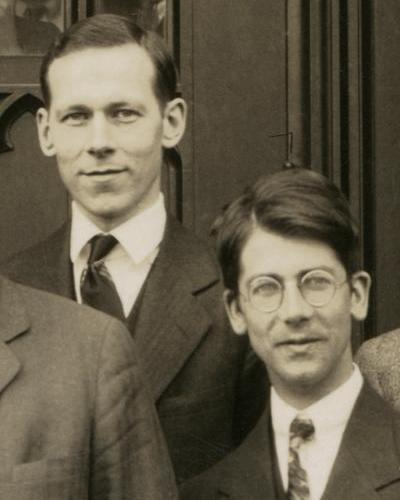
\includegraphics[width=\linewidth]{images/book3/mulliken-hund.jpg}
\end{minipage}\hfill
\begin{minipage}[t]{0.69\linewidth}
\vspace{0pt}
Antara tahun 1926 dan 1932, Friedrich Hund dan Robert Mulliken menafsirkan
spektrum molekul-molekul diatomik dengan menempatkan setiap elektron pada
sebuah orbital milik seluruh molekul, yang digolongkan menurut simetrinya
terhadap sumbu. Istilah $\sigma$, $\pi$, ikatan dan antiikatan, serta
diagram orbital dalam bab ini berasal dari karya mereka; Mulliken menerima
Hadiah Nobel Kimia pada tahun 1966. Foto ini menunjukkan Mulliken (kiri)
dan Hund di Chicago pada tahun 1929. (Foto: GFHund, CC BY 3.0, Wikimedia
Commons.)
\end{minipage}
\end{history}

\section{Ionisasi dan kekuatan ikatan}

Mengambil sebuah elektron dari \omterm{def:b2:diatomic-mos:bonding}{orbital ikatan} melemahkan ikatan;
mengambilnya dari \omterm{def:b2:diatomic-mos:bonding}{orbital antiikatan} memperkuatnya. Energi disosiasi
ion-ion diperoleh dari siklus termokimia: untuk
$\mathrm{AB}^+ \to \mathrm A + \mathrm B^+$,
\[
  D_0(\mathrm{AB}^+) = D_0(\mathrm{AB}) + I(\mathrm B) - I(\mathrm{AB}) ,
\]
dengan B atom yang energi ionisasinya lebih rendah.

\begin{example}[Ion-ion nitrogen dan oksigen]\label{ex:b2:diatomic-mos:ions}
\ce{N2} ($I = \qty{15.58}{eV}$) kehilangan elektron ikatan:
$D_0(\ce{N2+}) = 9.76 + 14.53 -
15.58 = \qty{8.71}{eV}$, lebih lemah
daripada \ce{N2}. \ce{O2} ($I = \qty{12.07}{eV}$) kehilangan elektron
$\pi^*$: $D_0(\ce{O2+}) = 5.12 + 13.62 - 12.07 = \qty{6.66}{eV}$, lebih kuat
daripada \ce{O2}, sesuai dengan \omterm{def:b2:diatomic-mos:bond-order}{orde ikatan} 2.5 dan 2.5 dibandingkan 3 dan
2.
% ledger: ie:N2, ie:N, ie:O2, ie:O, janafH0:N, janafH0:O
\end{example}

\section{Latihan}

\begin{exercise}[$\star$]\label{exo:b2:diatomic-mos:1}
Untuk dua orbital 1s hidrogen, ambillah $\alpha = \qty{-13.6}{eV}$,
$\beta = \qty{-9.0}{eV}$, dan $S = 0.60$ (data latihan). Hitunglah $E_+$ dan
$E_-$, lalu energi kedua elektron \ce{H2} dibandingkan dengan dua atom yang
terpisah.
\end{exercise}

\begin{exercise}[$\star$]\label{exo:b2:diatomic-mos:2}
Berikan \omterm{def:b2:diatomic-mos:bond-order}{orde ikatan} \ce{He2}, \ce{He2+}, \ce{Li2}, dan \ce{B2} (dengan
pencampuran s--p).
\end{exercise}

\begin{exercise}[$\star$]\label{exo:b2:diatomic-mos:3}
Manakah di antara \ce{B2}, \ce{C2}, \ce{N2}, \ce{O2}, \ce{F2} yang \omterm{def:b2:diatomic-mos:magnetism}{paramagnetik}?
\end{exercise}

\begin{exercise}[$\star$]\label{exo:b2:diatomic-mos:4}
Sumbu molekulnya adalah $z$. Pasangan manakah di antara (1s, $2\mathrm p_z$),
(1s, $2\mathrm p_x$), ($2\mathrm p_x$, $2\mathrm p_x$), ($2\mathrm p_x$,
$2\mathrm p_y$), (2s, $2\mathrm p_z$) yang tumpang-tindihnya tak nol?
\end{exercise}

\begin{exercise}[$\star\star$]\label{exo:b2:diatomic-mos:5}
Ramalkan apakah \ce{N2+} mempunyai ikatan yang lebih panjang atau lebih
pendek daripada \ce{N2}, lalu periksalah dengan energi disosiasinya yang
dihitung dalam bab ini.
\end{exercise}

\begin{exercise}[$\star\star$]\label{exo:b2:diatomic-mos:6}
Karbon monoksida dan \ce{N2} isoelektronik. Jelaskan mengapa
orbital-orbital ikatan CO berbobot pada oksigen dan mengapa orbital terisi
tertingginya merupakan pasangan elektron bebas pada karbon.
\end{exercise}

\begin{exercise}[$\star\star$]\label{exo:b2:diatomic-mos:7}
Dalam HF, orbital-orbital fluor manakah yang berinteraksi dengan 1s
hidrogen, dan manakah yang tetap nonikatan? Gambarlah diagramnya.
\end{exercise}

\begin{exercise}[$\star\star$]\label{exo:b2:diatomic-mos:8}
Dengan $\alpha_A = \qty{-10}{eV}$, $\alpha_B = \qty{-14}{eV}$, dan
$\beta = \qty{-3.0}{eV}$ (data latihan, $S$ diabaikan), hitunglah kedua
energi dan bobot $c_B^2$ \omterm{def:b2:diatomic-mos:bonding}{orbital ikatan} pada B.
\end{exercise}

\begin{exercise}[$\star\star$]\label{exo:b2:diatomic-mos:9}
Dengan pencampuran s--p, tunjukkan bahwa \ce{C2} mempunyai \omterm{def:b2:diatomic-mos:bond-order}{orde ikatan} 2
yang terdiri atas dua ikatan $\pi$ tanpa ikatan $\sigma_{2p}$.
\end{exercise}

\begin{exercise}[$\star\star\star$]\label{exo:b2:diatomic-mos:10}
Berikan \omterm{def:b2:diatomic-mos:bond-order}{orde ikatan} NO dan \ce{NO+}. Dari $D_0(\ce{NO}) = \qty{6.51}{eV}$,
$I(\ce{NO}) =
\qty{9.26}{eV}$, dan $I(\ce{O}) = \qty{13.62}{eV}$, hitunglah
$D_0(\ce{NO+})$ untuk $\ce{NO+} \to
\ce{N} + \ce{O+}$, lalu berilah
komentar.
\end{exercise}

\begin{exercise}[$\star\star\star$]\label{exo:b2:diatomic-mos:11}
Tunjukkan bahwa $E_+ + E_- = 2(\alpha - \beta S)/(1 - S^2)$, dan bahwa nilai
itu melampaui $2\alpha$ jika $\beta < \alpha S < 0$. Simpulkan mengapa dua
orbital yang terisi saling menolak (destabilisasi empat elektron).
\end{exercise}

\begin{exercise}[$\star\star\star$]\label{exo:b2:diatomic-mos:12}
Urutkan \ce{O2+}, \ce{O2}, \ce{O2-}, \ce{O2^2-} menurut \omterm{def:b2:diatomic-mos:bond-order}{orde ikatan}, panjang
ikatan, dan kekuatan ikatan. Ion manakah yang terdapat dalam hidrogen
peroksida, dan manakah yang terdapat dalam senyawa kuning \ce{KO2}?
\end{exercise}

\section{Soal: Oksigen dan Ion-ionnya}

\begin{problem}[{Soal akhir pekan --- diagram orbital molekul dioksigen,
orde ikatan dan kemagnetan ion-ionnya, ionisasi dan kekuatan ikatan, serta
dua cara memasangkan elektron-elektron $\pi^*$}]
\label{pb:b2:diatomic-mos:1}
Data: $I(\ce{O}) = \qty{13.62}{eV}$, $I(\ce{O2}) = \qty{12.07}{eV}$,
$I(\ce{N}) =
\qty{14.53}{eV}$, $I(\ce{N2}) = \qty{15.58}{eV}$;
$\Delta_f H_0$ pada \qty{0}{K} (\unit{kJ/mol}): \ce{O} 246.79, \ce{N}
470.82; $r_e$: \ce{O2} \qty{120.8}{pm}, \ce{N2} \qty{109.8}{pm};
$1\ \unit{eV} = \qty{96.485}{kJ/mol}$.
% ledger: ie:O, ie:O2, ie:N, ie:N2, janafH0:O, janafH0:N, re:O2, re:N2

\medskip
\noindent\textbf{Bagian I --- Dioksigen.}
\begin{enumerate}
  \item Berapa elektron valensi yang dimiliki \ce{O2}?
  \item Gambarlah diagram OM valensinya (tanpa pencampuran s--p) dan
        isilah.
  \item Hitunglah \omterm{def:b2:diatomic-mos:bond-order}{orde ikatannya}.
  \item Berapa elektron tak berpasangan? Apakah \ce{O2} \omterm{def:b2:diatomic-mos:magnetism}{paramagnetik}?
  \item Mengapa struktur Lewis gagal di sini?
  \item Hitunglah $D_0(\ce{O2})$ dalam \unit{eV}.
\end{enumerate}

\medskip
\noindent\textbf{Bagian II --- Ion-ion.}
\begin{enumerate}[resume]
  \item Berikan konfigurasi dan \omterm{def:b2:diatomic-mos:bond-order}{orde ikatan} \ce{O2+}.
  \item Hal yang sama untuk ion superoksida \ce{O2-}.
  \item Hal yang sama untuk ion peroksida \ce{O2^2-}.
  \item Berikan jumlah elektron tak berpasangan setiap ion.
  \item Urutkan \ce{O2+}, \ce{O2}, \ce{O2-}, \ce{O2^2-} menurut panjang
        ikatan yang diramalkan.
  \item Ion manakah yang mempunyai ikatan tunggal O--O, seperti hidrogen
        peroksida?
  \item Manakah dari keempat spesies itu yang \omterm{def:b2:diatomic-mos:magnetism}{paramagnetik}?
\end{enumerate}

\medskip
\noindent\textbf{Bagian III --- Ionisasi.}
\begin{enumerate}[resume]
  \item Dari orbital mana elektron pergi ketika \ce{O2} diionisasi?
  \item Mengapa $I(\ce{O2})$ lebih rendah daripada $I(\ce{O})$?
  \item Tunjukkan bahwa $D_0(\ce{O2+}) = D_0(\ce{O2}) + I(\ce{O}) - I(\ce{O2})$
        lalu hitunglah nilainya.
  \item Bandingkan dengan $D_0(\ce{O2})$ dan jelaskan.
  \item Hitunglah $D_0(\ce{N2})$ dan $D_0(\ce{N2+})$ dengan cara yang sama.
  \item Mengapa $I(\ce{N2})$ lebih tinggi daripada $I(\ce{N})$?
  \item Simpulkan: kapan ionisasi memperkuat sebuah ikatan?
\end{enumerate}

\medskip
\noindent\textbf{Bagian IV --- Elektron-elektron $\pi^*$.}
\begin{enumerate}[resume]
  \item Dalam keadaan dasar, kedua elektron $\pi^*$ menempati dua orbital
        yang berbeda dengan spin sejajar. Aturan manakah yang menyatakan
        hal itu?
  \item Uraikan suatu keadaan ketika keduanya menempati orbital $\pi^*$
        yang sama.
  \item Mengapa keadaan itu energinya lebih tinggi?
  \item Berapa \omterm{def:b2:diatomic-mos:bond-order}{orde ikatan} dan bagaimana kemagnetannya?
  \item Nyatakan \omterm{def:b2:diatomic-mos:bond-order}{orde ikatan} \ce{O2+} dan energi disosiasinya.
\end{enumerate}
\end{problem}
